\documentclass[jou]{apa6}

\usepackage[american]{babel}

\usepackage{csquotes}
\usepackage[style=apa,sortcites=true,sorting=nyt,backend=biber]{biblatex}
\DeclareLanguageMapping{american}{american-apa}
\addbibresource{bibliography.bib}


%%%%%%%%%%%%%%%%%%%%%%%%%%%%%%%%%%%%%%%%
%% Discrete Structures
%% The start of RBS stuff
%%%%%%%%%%%%%%%%%%%%%%%%%%%%%%%%%%%%%%%%

% Working internal and external links in PDF
\usepackage{hyperref}
% Extra math symbols in LaTeX
\usepackage{amsmath}
\usepackage{gensymb}
\usepackage{amssymb}
% Enumerations with (a), (b), etc.
\usepackage{enumerate}
\usepackage[framemethod=TikZ]{mdframed}
\usepackage{xcolor}

\let\OLDitemize\itemize
\renewcommand\itemize{\OLDitemize\addtolength{\itemsep}{-6pt}}

\usepackage{etoolbox}
\makeatletter
\preto{\@verbatim}{\topsep=3pt \partopsep=3pt }
\makeatother

% These sizes redefine APA for A4 paper size
\oddsidemargin 0.0in
\evensidemargin 0.0in
\textwidth 6.27in
\headheight 1.0in
\topmargin -24pt
\headheight 12pt
\headsep 12pt
\textheight 9.19in



\title{Sample Quiz 8}
\author{Discrete Structures, Spring 2020}
\affiliation{RBS}

\leftheader{Discrete Sample Quiz 8}

\abstract{%
}

%\keywords{}

\setlength\parindent{0pt}

\begin{document}

\thispagestyle{empty}

\twocolumn
{\Large Quiz 12 (Trees)}

{\bf Question 1.} The wheel graph $W_4$ has $5$ vertices: 
$4$ vertices form a cycle graph $C_4$ \textendash{} a square; 
one more vertex sits in the middle and is connected with the remaining $4$ vertices. 
($W_4$ is isomorphic to an ordinary Egyptian pyramid.) 
Assume that all vertices in the wheel graph are named with letters and are distinguishable. 
Find the number of unrooted spanning trees in the $W_4$.\\
Write a positive integer in your answer.

\vspace{10pt}
{\bf Question 2.} It is known that a full $m$-ary tree $T$ has $25$ leaves, but the parameter $m$ is 
not known \textendash{} it can take any fixed value: $m = 2,3,4,\ldots$. 
How many inner nodes can $T$ have? Find all possible answers.\\
Write an increasing comma-separated list.

\vspace{10pt}
{\bf Question 3.}\\ There is a rooted tree with $111$ vertices and each vertex can have up to $3$ children. 
Find the minimum and the maximum height of this tree.\\
Write two comma-separated integers.


\vspace{10pt}
{\bf Question 4.}\\ 
Assume that there is a rooted tree (with anonymous/unnamed vertices and unordered children) and its vertices have 
the following degrees $3, 3, 2, 2, 1, 1, 1, 1$. It is also known that its root vertex has $3$ children. 
Find the number of such rooted unordered trees.\\
Write a positive integer.


\vspace{10pt}
{\bf Question 5.}
\begin{center}
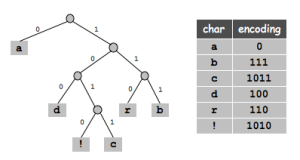
\includegraphics[width=3.2in]{huffman-tree.png}\\
{\em Figure 1: Encoding with a Tree}
\end{center}
The given tree shows an efficient method send messages
(like {\tt abracadabra!}) using $6$ characters.
Assume that the characters appear with the following probabilities:\\
{\small
\begin{tabular}{|l|c|c|c|c|c|c|} \hline
Symbol & {\tt a} & {\tt b} & {\tt d} & {\tt r} & {\tt c} & {\tt !} \\ \hline
Probability &  $1/2$ & $1/8$ & $1/8$ & $1/8$ & $1/16$ & $1/16$ \\ \hline
\end{tabular}\\
}
Find the expected number of bits used per character (i.e. $E(X)$ \textendash{} the expected value of
the random variable $X$, which describes the number of bits used per one
character from this random distribution.)\\
Write a real number \textendash{} the number of bits rounded to the nearest thousandth.

%{\em Note.} For the given probabilities, this tree offers the best compression
%(using it for the encoding needs the smallest 
%expected number of bits). For such optimal codes we say that the expected number of bits
%for sending one character equals the {\em entropy} of the probability distribution.
%It is fine, if the entropy is a fractional (non-integer) number of bits.



 
 


\vspace{10pt}
{\bf Question 6.} 
The string
$$\rightarrow\;\rightarrow\;\rightarrow\;\rightarrow\;\rightarrow\;a\;b\;\textcolor{red}{\triangle}\;\neg\;c\;\neg\;d\;c\;e\;\rightarrow\;\neg\;a\;\rightarrow\;d\;e.$$
is the prefix notation for a Boolean logic expression with one symbol replaced by a $\textcolor{red}{\triangle}$. 
What can this $\textcolor{red}{\triangle}$ represent?\\
{\bf (A)} It is a propositional variable ($a,b,c$ or similar).\\
{\bf (B)} It is a unary Boolean operator ($\neg$ or similar).\\
{\bf (C)} It is a binary Boolean operator ($\rightarrow$ or similar).\\
{\bf (D)} It cannot be any of these; the expression is invalid in all these cases.

Write the answer letter (A, B, C, or D).



\vspace{10pt}
{\bf Question 7.} 
Imagine that you search for all ways how to place $4$ queens on a $4 \times 4$ chessboard so that 
they do not attack each other. (A chess queen attacks all squares on its horizontal, on its vertical
and also on both diagonals.)\\
Imagine that you build a tree for this:\\
{\bf (Level 0 to Level 1)} The root of the tree is an empty $4 \times 4$ chess-board; you add to it four children 
(all $4$ ways how you can place a queen on the 1st row of the chess-board).\\
{\bf (Level 1 to Level 2)} For any of the vertices you added in the previous step, add children on level $2$ by placing 
another queen on the 2nd row so that it does not attack the first one.\\
In general, the vertex on level $L=i$ has queens on rows $1,\ldots,i$ that do not attack each other. 
Any vertex on level $L=4$ will be a solution to this ``4 queens problem'' with all four rows containing a queen.

Write the total number of vertices in this tree (that the backtracking algorithm will visit).


\vspace{10pt}
{\bf Question 8.} An undirected graph $G = (V,E)$ has the set of vertices $V$ \textendash{} 
the set of all positive divisors of the number $900$ (including $1$ and $900$ itself).
A pair of divisors $(d_1,d_2)$ is an edge in $G$ iff their ratio
$d_1/d_2$ (or $d_2/d_1$) is a prime number.

In the root vertex $v_1=1$ we start the BFS (Breadth-first-search) traversal of the graph $G$. For every vertex 
we visit all its adjacent vertices in increasing order (for example edges $(1,2)$, $(1,3)$ and $(1,5)$ 
are visited in this order. When all the children of vertex $1$ are visited, 
we start visiting all the adjacent vertices of $v_2=2$, and so on.). We get the BFS traversal order like this:
$$v_1=1,\,v_2=2,\,v_3=3,\,v_4=5,\,v_5=4,\,\ldots$$
Find the vertices $v_{13},\,v_{14},\,v_{15}$ in this BFS order.

Write three comma-separated numbers.

\newpage
%\vspace{10pt}
{\bf Question 9.}
\begin{center}
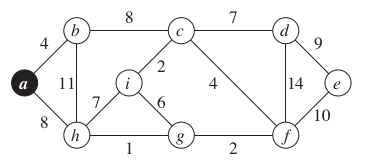
\includegraphics[width=2in]{prim-algorithm.png}\\
{\em Figure 2: Weighted Graph}
\end{center}
Find the weight of a minumum spanning tree (MST) in the given tree. 
In order to construct this tree, you can use Prim's algorithm (Rosen2019, p.836). 
Start in vertex $a$ - this is your first tree $T_1$. 
In every step pick the minimum weight edge that is adjacent to $T_i$ (and does 
not create any loop) \textendash{} add it to the tree $T_i$, and obtain the next 
tree $T_{i+1}$. Continue adding the minimum weight edges until all vertices are connected.
(In the second step you will have a choice 
to add $(b,c)$ or $(a,h)$ as both edges have the same weight $8$. There may be several MSTs
in a graph, but all of them will have the same total weight.)

Write the total MST weight as a number.



\vspace{4pt}
{\bf Question 10.}
\begin{center}
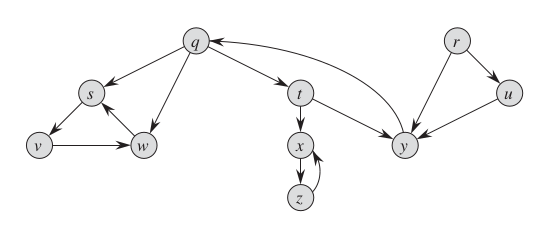
\includegraphics[width=3in]{dfs-traversal2.png}\\
{\em Figure 3: Graph for DFS traversal}
\end{center}

The vertices in the above directed graph are visited in the DFS
order. You start with the alphabetically smallest vertex ($q$), order all the vertices connected to it
alphabetically, then build the DFS traversal. 

Write the sequence with parentheses and vertices for the graph 
on \textcolor{red}{Figure 3} \textendash{} similar to the sequence (\ref{eq1}) \textendash{} see Appendix. 
Each of its $10$ vertices should be mentioned in your 
traversal order twice (the first time with an opening parenthesis, the second time 
with a closing parenthesis).






\vspace{20pt}
\section{Appendix: DFS}

%\begin{mdframed}[roundcorner=6pt]
\begin{center}
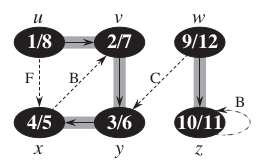
\includegraphics[width=1.4in]{dfs-traversal.png}\\
{\em Figure 4: Sample DFS traversal}
\end{center}
Figure 4 shows a DFS (Depth-First-Search) traversal
in a directed graph. Vertexes are visited in alphabetical order 
(so $u$ is visited first; followed by its alphabetically first 
child $v$, followed by $y$, followed by $x$. After that
we visit another tree (unreachable from the first one) \textendash{}
$w$ followed by $z$.)\\
{\bf Tree edges} that belong to the DFS traversal tree are shaded;\\
{\bf Back edges} that point back from a vertex to its ancestor in the tree (or a loop to itself)
are labeled by $B$;\\
{\bf Forward edges} that jump from a vertex to its descendant in the DFS tree (other than a child) are
labeled by $F$;\\
{\bf Cross edges} that jump between two vertices that are not descendants/ancestors of 
each other are labeled by $C$.

The following sequence
\begin{equation} \label{eq1}
\textcolor{blue}{\mathtt{(u\;(v\;(y\;(x\;x)\;y)\;v)\;u)\;(w\;(z\;z)\;w)}}
\end{equation}
denotes the DFS traversal order in the oriented graph. 
Every time when we enter some vertex (and its subtree), 
we open a parenthesis and write the vertex name; when we leave, 
we write the vertex name again and close the parenthesis.\\
This order is also written inside each vertex (for example {\tt 1/8} 
for vertex $u$ means that we entered it in Step 1, and left it in 
Step 8). For vertex $z$ this pair is {\tt 10/11} (we entered this leaf
of the DFS tree and immediately left it).
%\end{mdframed}


%\begin{mdframed}[roundcorner=6pt]
%\section{Appendix 2: Prim's Algorithm}

%\end{mdframed}

\end{document}

